% -*- root: ../main.tex -*-
%!TEX root = ../main.tex
% vim:textwidth=80 fo=cqt

\backmatter
\singlespacing
\begin{footnotesize} % Bibliography/References
    \renewcommand{\bibname}{References} % changes the header; default: Bibliography
    % add bib to toc
    \cleardoublepage
    \phantomsection
    \addcontentsline{toc}{chapter}{\bibname}
    \newgeometry{bottom=1.1in} % https://tex.stackexchange.com/questions/161773/top-margin-of-bibliography
    \printbibliography[notcategory=ignore]
    \restoregeometry
\end{footnotesize}

% Required to maintain continuous arabic numbering
\makeatletter
\@mainmattertrue
\makeatother
\cleardoublepage


% \setstretch{1.348361657291667} % golden-ratio stretch (1.2 x 1.348 = 1.618)
\begin{appendices} % Using the appendices environment (from appendix package) for more functionality
    \crefalias{chapter}{appchap}
    % -*- root: ../../main.tex -*-
%!TEX root = ../../main.tex
% vim: nospell

% ******************************* Thesis Appendix A ****************************
\chapter{Full Listing of Program Codes}
\startcontents[chapters]
\printcontents[chapters]{}{1}{\setcounter{tocdepth}{1}}

\cleardoublepage
\fakesection{MATLAB codes for continuous-time SPM}

\glsdisablehyper
\matlabcodelisting[\textsc{MATLAB} code for simulation of continuous time SPM]{backmatter/appendices/matlab_codes/cts_time_spm_simulation.m}{sc:ctstimespm}

\cleardoublepage
\fakesection{MATLAB codes for discrete-time SPM}
\matlabcodelisting[\textsc{MATLAB} code for simulation of discrete time SPM]{backmatter/appendices/matlab_codes/disc_time_spm_simulation_massive.m}{sc:disctimespm}

\glsenablehyper

% graphviz doc in appendix, toolbox, directory listing etc.

    % -*- root: ../../main.tex -*-
%!TEX root = ../../main.tex
% vim: nospell

% ******************************* Thesis Appendix A ****************************
\chapter{Permissions Summary}\label{ch:permissions}
\startcontents[chapters]
\printcontents[chapters]{}{1}{\setcounter{tocdepth}{1}}

\cleardoublepage
\fakesection{Summary of Copyright Permissions}
% -*- root: ../../main.tex -*-
%!TEX root = ../../main.tex

% \pagestyle{empty}
\begin{landscape}
    \makeatletter \PLS@RemoveRotate % from chat with Ulrike Fischer
    \centering
    \begin{footnotesize}
        \begingroup
        % \setlength{\tabcolsep}{5pt}
        \renewcommand{\arraystretch}{1.5}
        \begin{longtable}[c]{@{} l  l p{7.5cm} l c c p{1.6cm} @{}}
            \caption{\normalsize Summary of permissions for reuse of third-party copyrighted material} \label{tbl:permissionstable} \\

            \toprule
            \multicolumn{1}{c}{\makecell{Page \\ no.}} & \makecell{Usage in \\ thesis} & \makecell{Source \\ \vphantom{of work}} & \makecell[l]{Copyright holder \& \\ contact (organisations only)} & \makecell{Permission \\ requested on} & \makecell{Have \\ permission?} & \makecell{Permission \\ remarks} \\
        \midrule
        \endfirsthead

        \multicolumn{7}{c}%
        {{\normalsize \bfseries \tablename\ \thetable{} --- \normalfont  continued from previous page}} \\
        \toprule
        \multicolumn{1}{c}{\makecell{Page \\ no.}} & \makecell{Usage in \\ thesis} & \makecell{Source \\ \vphantom{of work}} & \makecell[l]{Copyright holder \& \\ contact (organisations only)} & \makecell{Permission \\ requested on} & \makecell{Have \\ permission?} & \makecell{Permission \\ remarks} \\
        \midrule
        \endhead

        \midrule
        \multicolumn{7}{ r @{}}{{\normalsize  Continued on next page}} \\[-1ex]
        \bottomrule
        \endfoot

        \bottomrule
       \endlastfoot

           \Cpageref{fig:energyvspowercell}         & \Cref{fig:energyvspowercell}          & \printpublication{VonSrbik2015}     & \Citeauthor*{VonSrbik2015}          & N/A                                                                & Yes                            & CC-BY-NC-ND                                           \\
           \Cpageref{fig:fig_CC_discharge_curves}   & \Cref{fig:fig_CC_discharge_curves}    & \printpublication{Gopalakrishnan2018}            & \makecell[lt]{Elsevier             \\ \href{mailto:permissions@elsevier.com}{permissions@elsevier.com}}  & \DTMdate{2018-12-26}                                               & No & Pending publishing agreement\\
           \Cpageref{fig:1d_fv_mesh}                & \Cref{fig:1d_fv_mesh}                 & \printpublication{Torchio2016}      & \makecell[lt]{The Electrochemical Society             \\ \href{mailto:copyright@electrochem.org}{copyright@electrochem.org}}& \DTMdate{2018-09-28}                                               & Yes                            & \mbox{`Rightslink'} service agreement attached               \\
           \Cpageref{fig:anodeoverhangpouchcell}    & \Cref{fig:anodeoverhangpouchcell}     & \printpublication{Bond2017}         & \Citeauthor{Bond2017}               & N/A                                                                & Yes                            & CC-BY                                                 \\
           \Cpageref{fig:topologies}                & \Cref{fig:topologies}                 & \printpublication{Northrop2011}     &  \makecell[lt]{The Electrochemical Society             \\ \href{mailto:copyright@electrochem.org}{copyright@electrochem.org}}           & \DTMdate{2018-09-27}                                               & Yes                            & \mbox{`Rightslink'} service agreement attached               \\
           \Cpageref{fig:fig_generate_heatmap_BEV}  & \Cref{fig:fig_generate_heatmap_BEV}   & \printpublication{Gopalakrishnan2018}            & \makecell[lt]{Elsevier             \\ \href{mailto:permissions@elsevier.com}{permissions@elsevier.com}}  & \DTMdate{2018-12-26}                                               & No & Pending publishing agreement \\
           \Cpageref{fig:fig_generate_heatmap_PHEV} & \Cref{fig:fig_generate_heatmap_PHEV}  & \printpublication{Gopalakrishnan2018}            & \makecell[lt]{Elsevier             \\ \href{mailto:permissions@elsevier.com}{permissions@elsevier.com}}  & \DTMdate{2018-12-26}                                               & No & Pending publishing agreement \\
           \Cpageref{fig:fig_CapacityQuadrants}     & \Cref{fig:fig_CapacityQuadrants}      & \printpublication{Gopalakrishnan2018}            & \makecell[lt]{Elsevier             \\ \href{mailto:permissions@elsevier.com}{permissions@elsevier.com}}  & \DTMdate{2018-12-26}                                               & No & Pending publishing agreement \\
           \Cpageref{ch:improveddra}                & \makecell[lt]{All figures,           \\ tables and                 \\ captions of                        \\ \cref{ch:improveddra}}                                             & \printpublication{Gopalakrishnan2017}  & \makecell[lt]{The American Society                    \\ of Mechanical Engineers   \\ (ASME)  \\ \href{mailto:copyright@asme.com}{copyright@asme.com}}  & \DTMdate{2016-04-19} & Yes & \makecell[lt]{Copyright \\ agreement} \\
           \Cpageref{fig:sandwichtospm}             & \Cref{fig:sandwichtospm}              & \printpublication{Moura2012}        & \makecell[lt]{The American Society \\ of Mechanical Engineers                                           \\ (ASME)                        \\ \href{mailto:copyright@asme.com}{copyright@asme.com}}  & \DTMdate{2018-09-25}       & Yes  & \mbox{`Rightslink'} service agreement attached                          \\ \Cpageref{fig:timingdiagramBig}          & \Cref{fig:timingdiagramBig}           & \fullcite{Southward2011}    & \Citeauthor*{Southward2011}         & \DTMdate{2018-09-26}                                               & Yes & Granted via email \\
           \Cpageref{fig:timingdiagramSmall}        & \Cref{fig:timingdiagramSmall}         & \printpublication{PlettECE5540_02}  & \Citeauthor*{PlettECE5540_02}       & \DTMdate{2018-09-28}                                               & Yes                            & Granted via email                                              \\
           \Cpageref{fig:coordsquadapprox}          & \Cref{fig:coordsquadapprox}           & \printpublication{Deng2018}         & \makecell[lt]{Elsevier             \\ \href{mailto:permissions@elsevier.com}{permissions@elsevier.com}}  & \DTMdate{2018-09-27}           & Yes                                                    & Elsevier license attached \\

        \end{longtable}
   \endgroup
    \end{footnotesize}
\end{landscape}


\makeatletter\@sc@wm@stampfalse\makeatother

\fakesection{Copyright Permissions for reuse of \Cref{fig:1d_fv_mesh}}
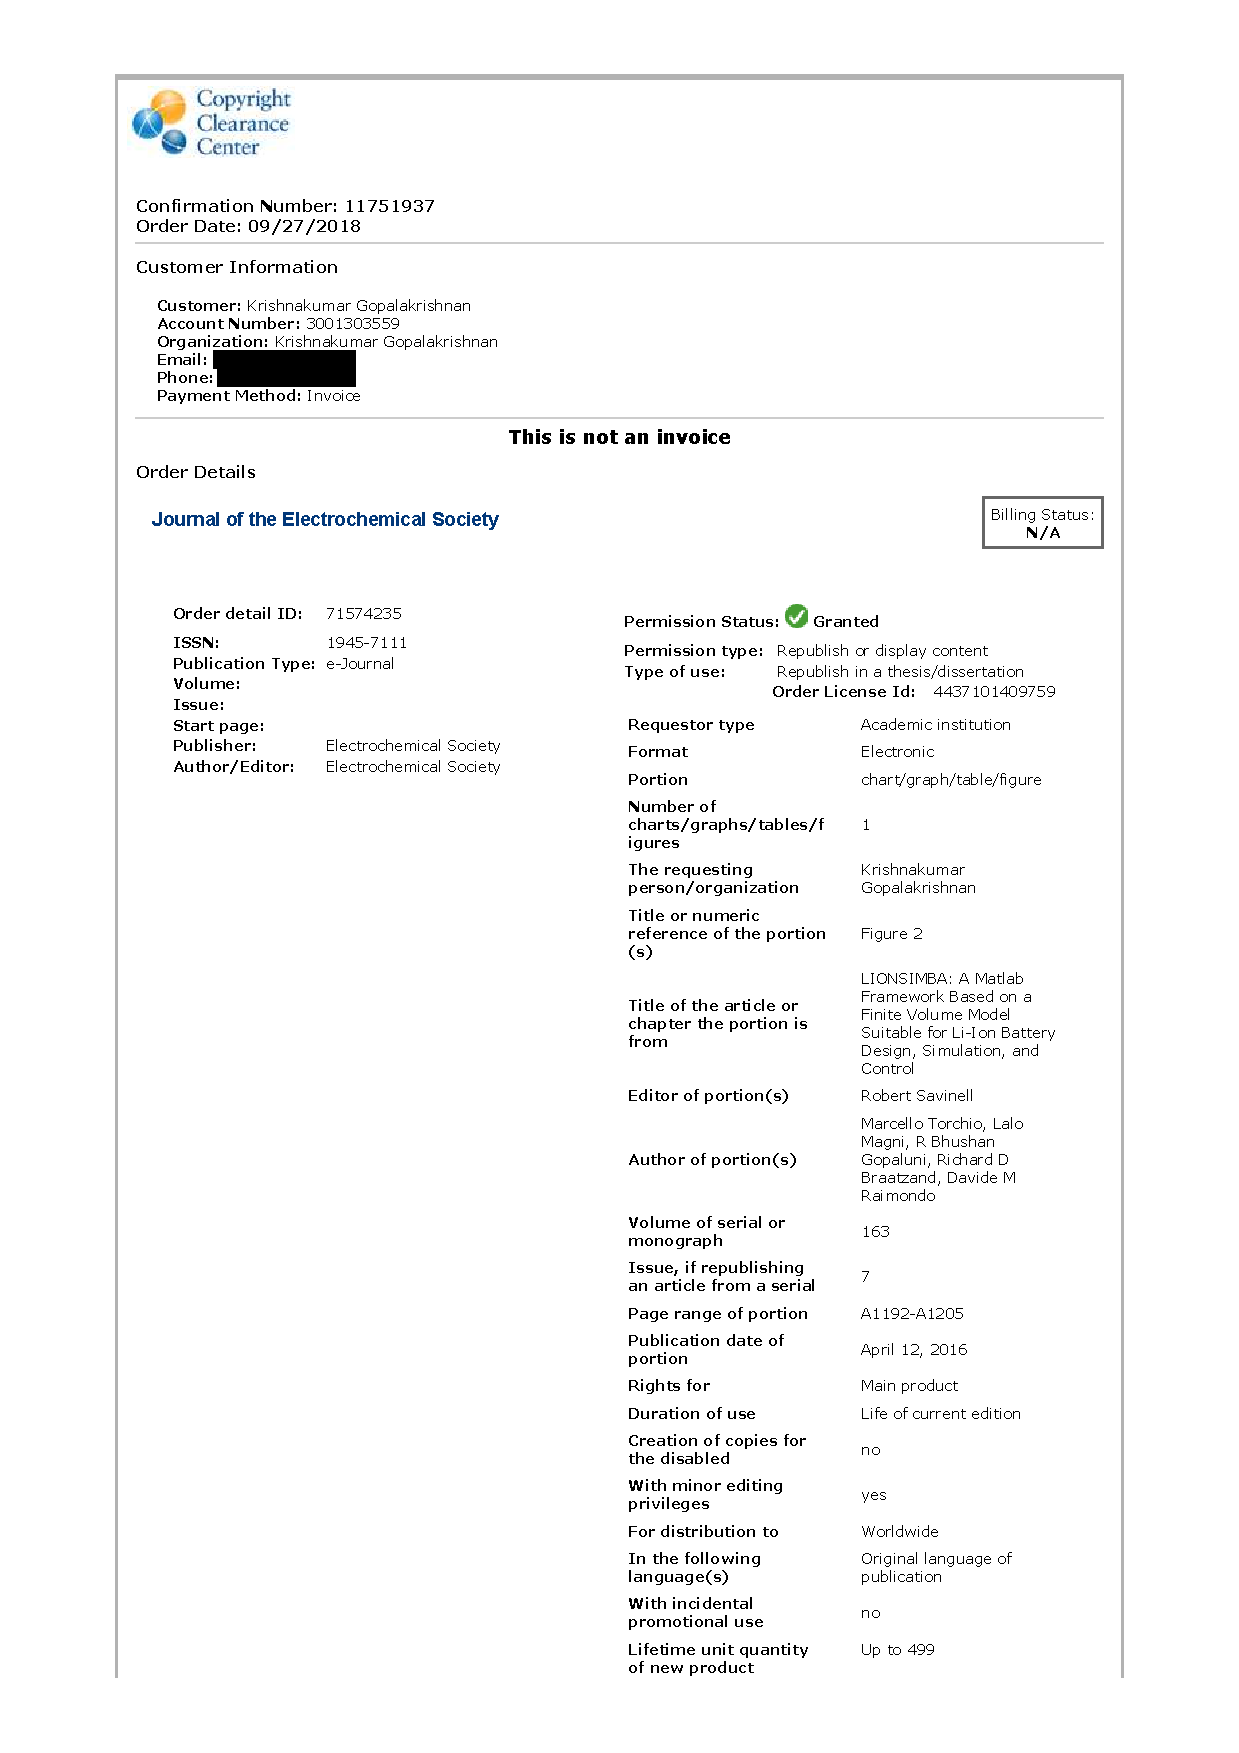
\includepdf[pages=-,scale=0.885,link,linkname=torchio,pagecommand={\label{torchiopermission}}]{backmatter/appendices/redacted_JES_Torchio_permission_pdf.pdf}
\fakesection{Copyright Permissions for reuse of \Cref{fig:topologies}}
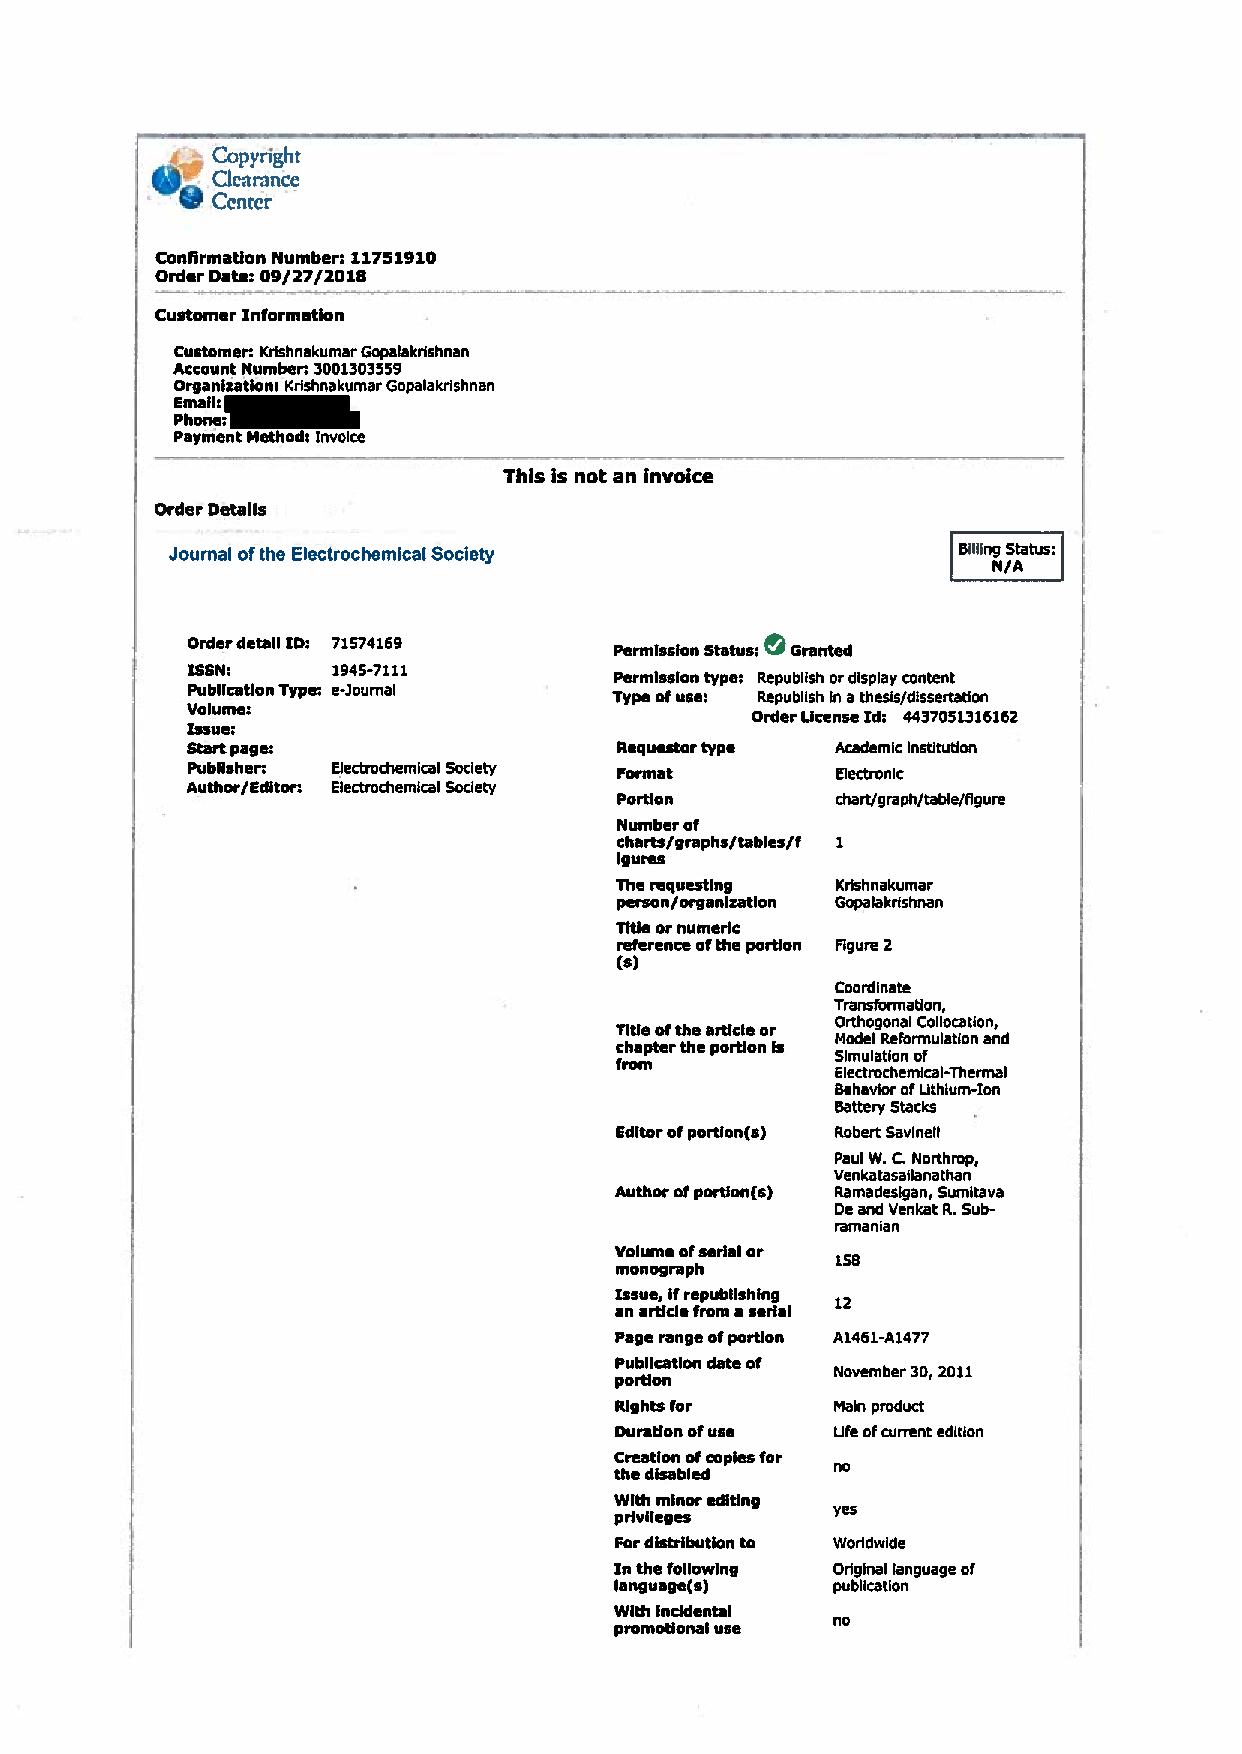
\includepdf[pages=-,scale=0.885,angle=0.1,link,linkname=northrop,pagecommand={\label{northroppermission}}]{backmatter/appendices/redacted_Northrop_permission_pdf.pdf}
\fakesection{Copyright Permissions for reuse of text, figures and tables of \Cref{ch:improveddra}}
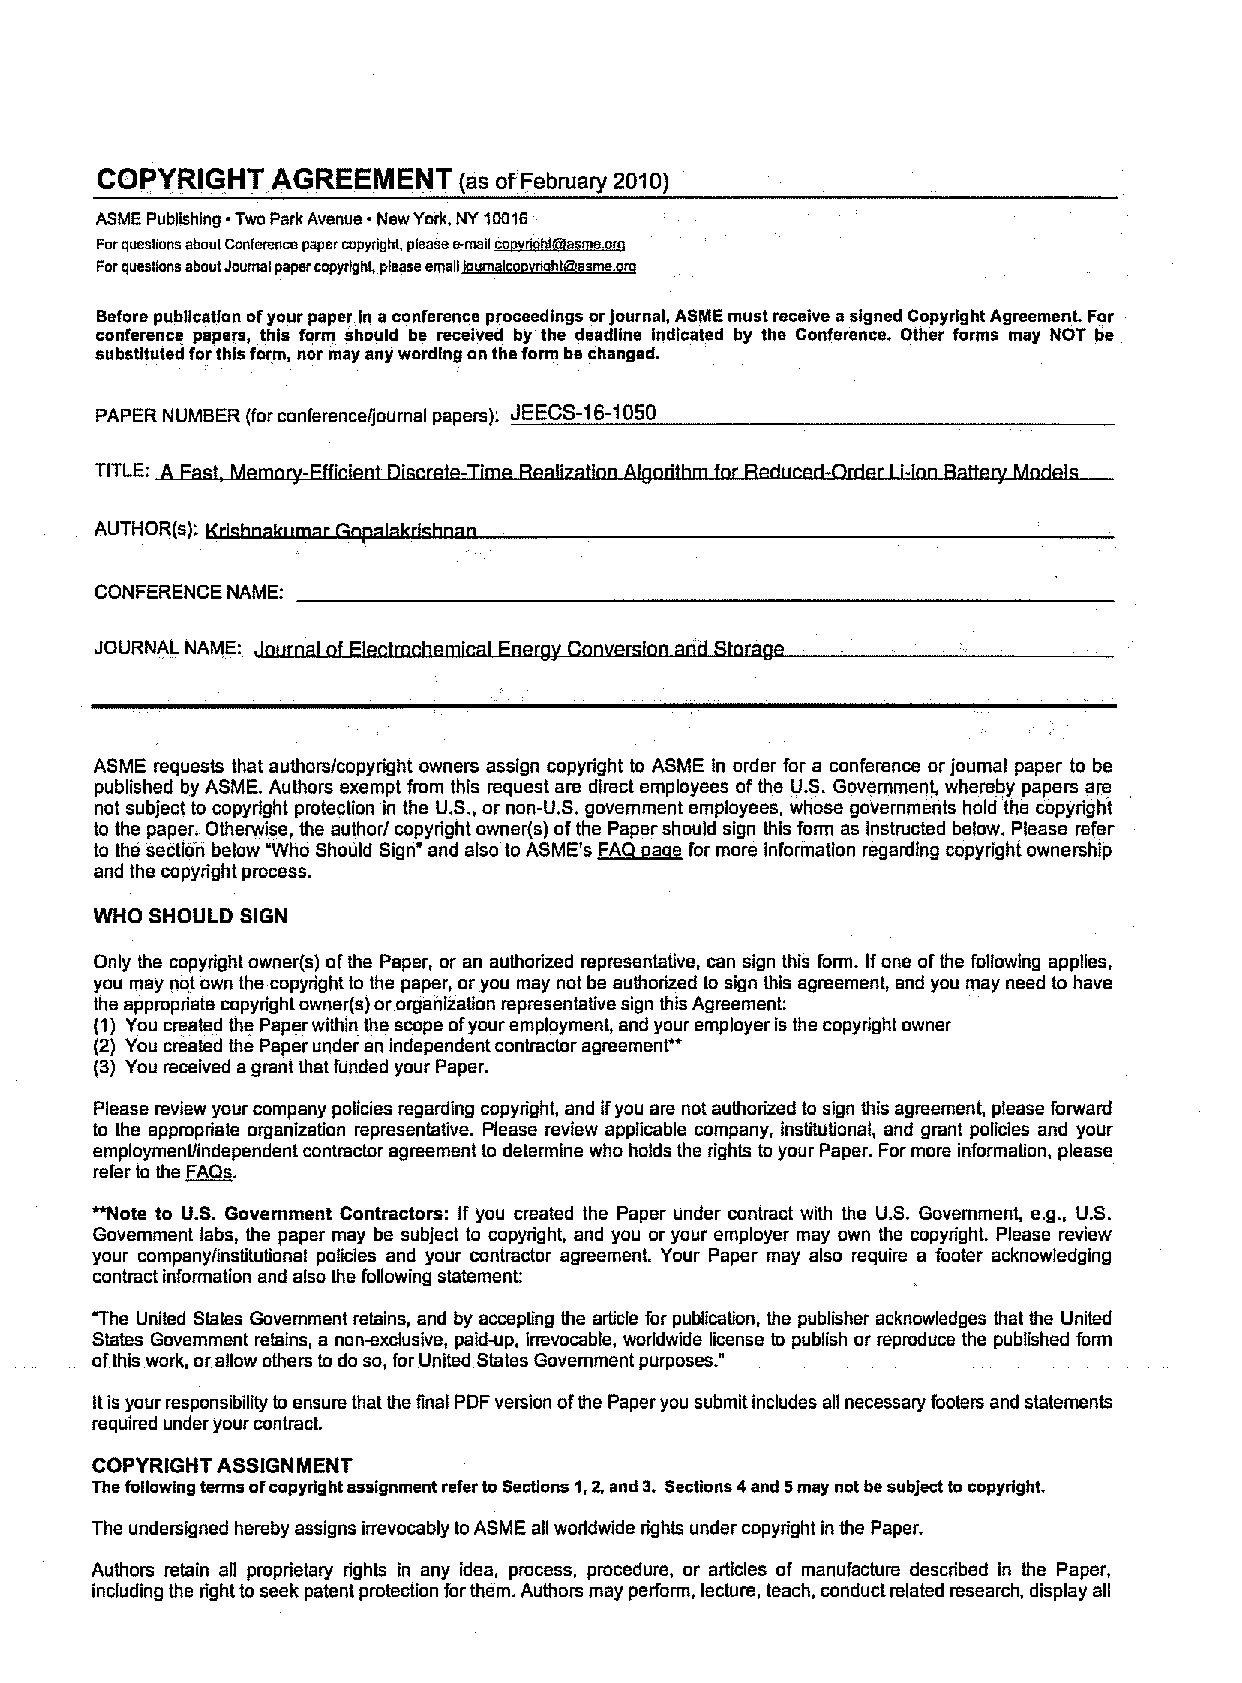
\includepdf[pages=-,scale=0.885,offset= 0in 0.35in,link,linkname=asme,pagecommand={\label{asmepermission}}]{backmatter/appendices/asme_copyright.pdf}
\fakesection{Copyright Permissions for reuse of \Cref{fig:sandwichtospm}}
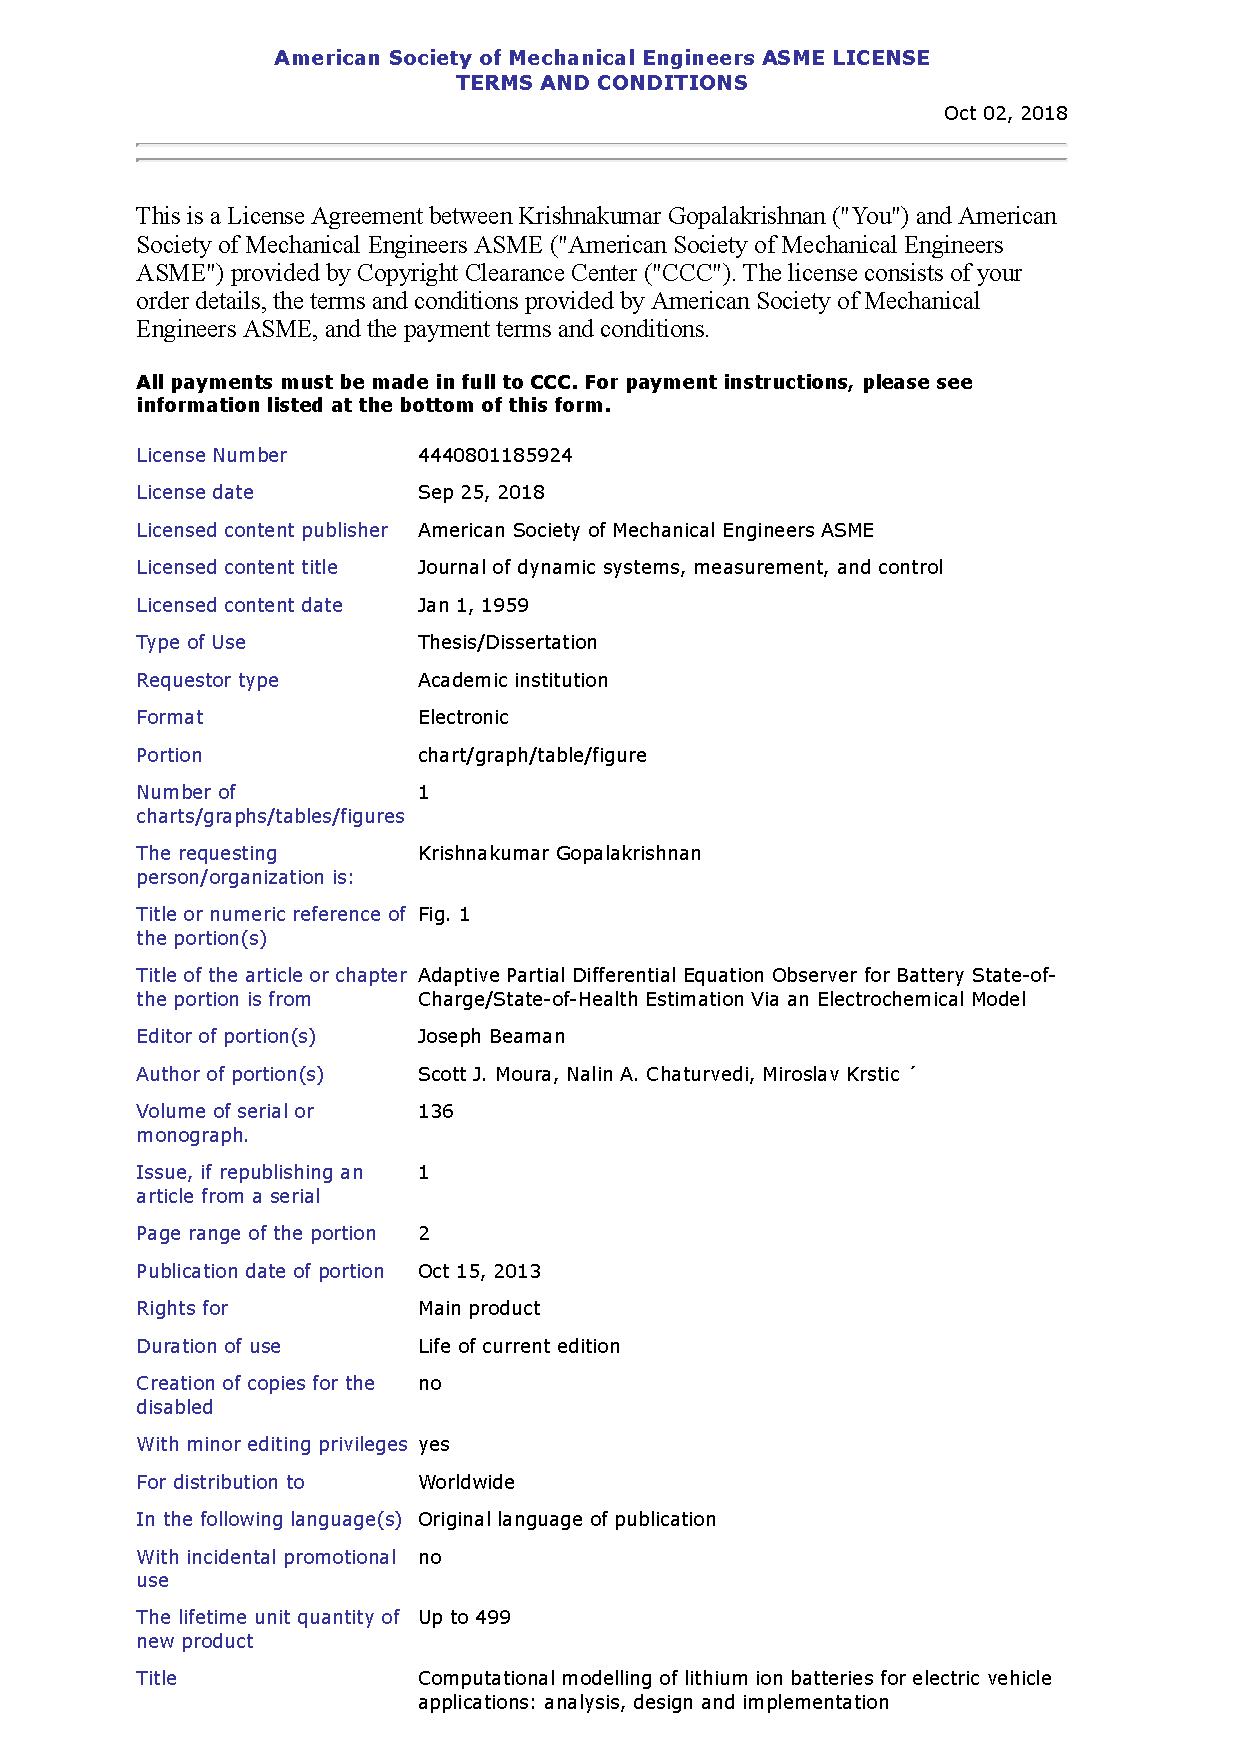
\includepdf[pages=-,scale=0.80,link,linkname=moura,pagecommand={\label{mourapermission}}]{backmatter/appendices/redacted_Moura_etal_permissions.pdf}
\fakesection{Copyright Permissions for reuse of \Cref{fig:timingdiagramBig}}
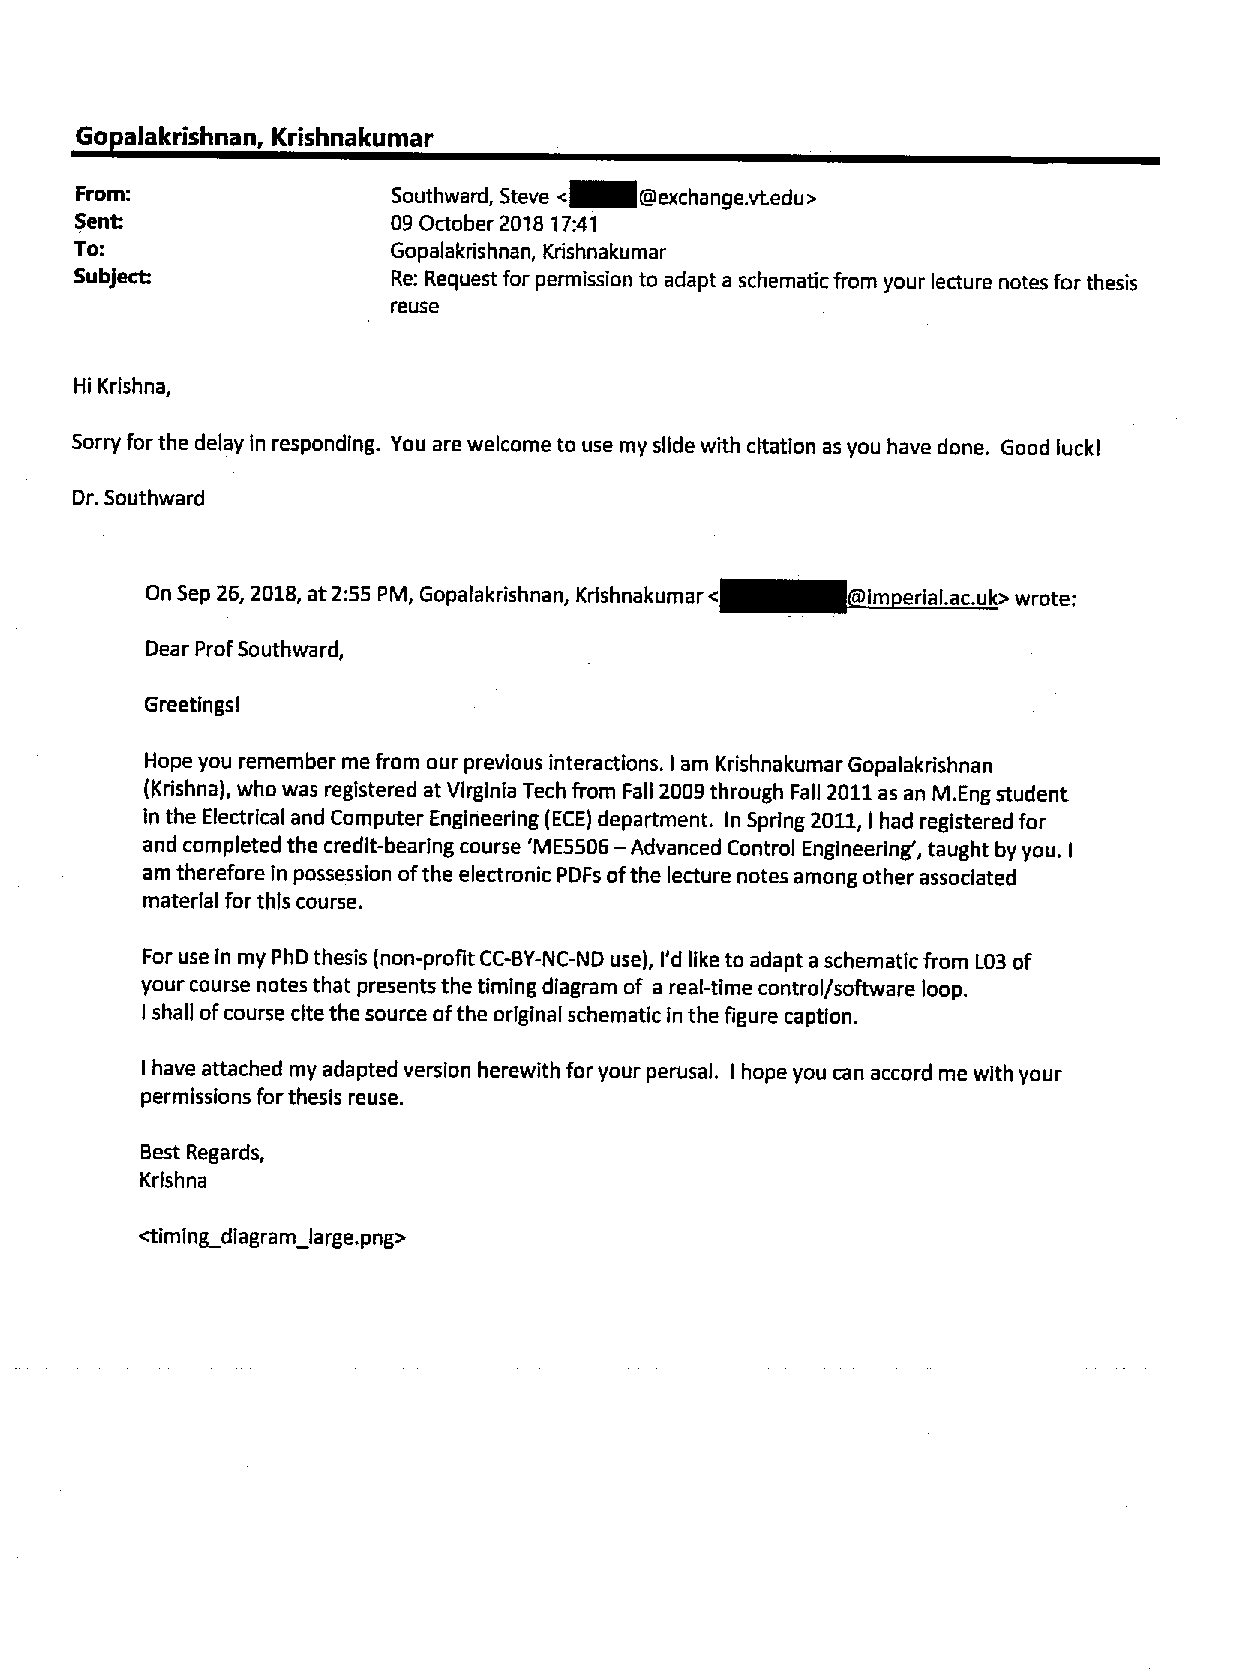
\includepdf[pages=-,scale=0.84,offset= 0in 0.45in,angle=0.44,link,linkname=southward,pagecommand={\label{southwardpermission}}]{backmatter/appendices/southward_redacted_OCRed_email.pdf}
\fakesection{Copyright Permissions for reuse of \Cref{fig:timingdiagramSmall}}
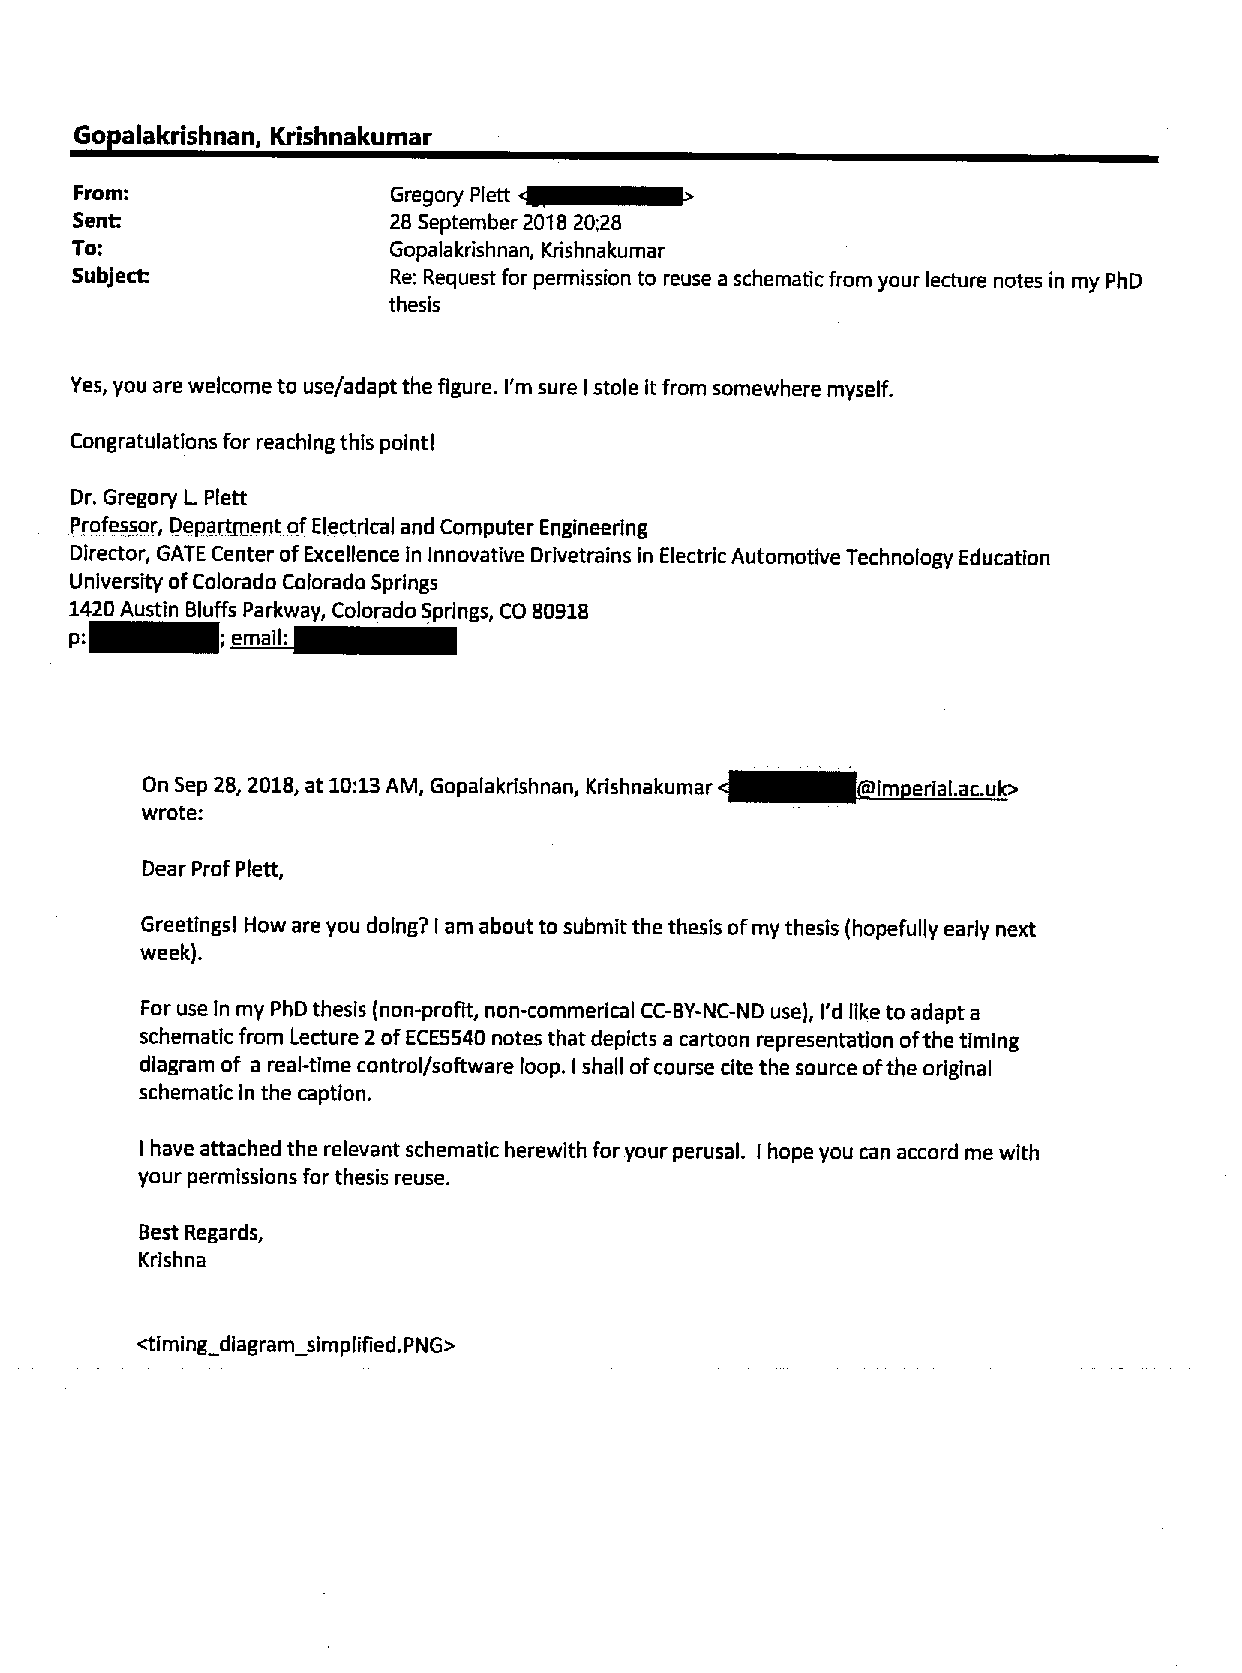
\includepdf[pages=-,scale=0.84,offset= 0in 0.45in,angle=0.44,link,linkname=plett,pagecommand={\label{plettpermission}}]{backmatter/appendices/plett_redacted_OCRed_email.pdf}
\fakesection{Copyright Permissions for reuse of \texorpdfstring{\Cref{fig:coordsquadapprox}}{Figure 5.14}}
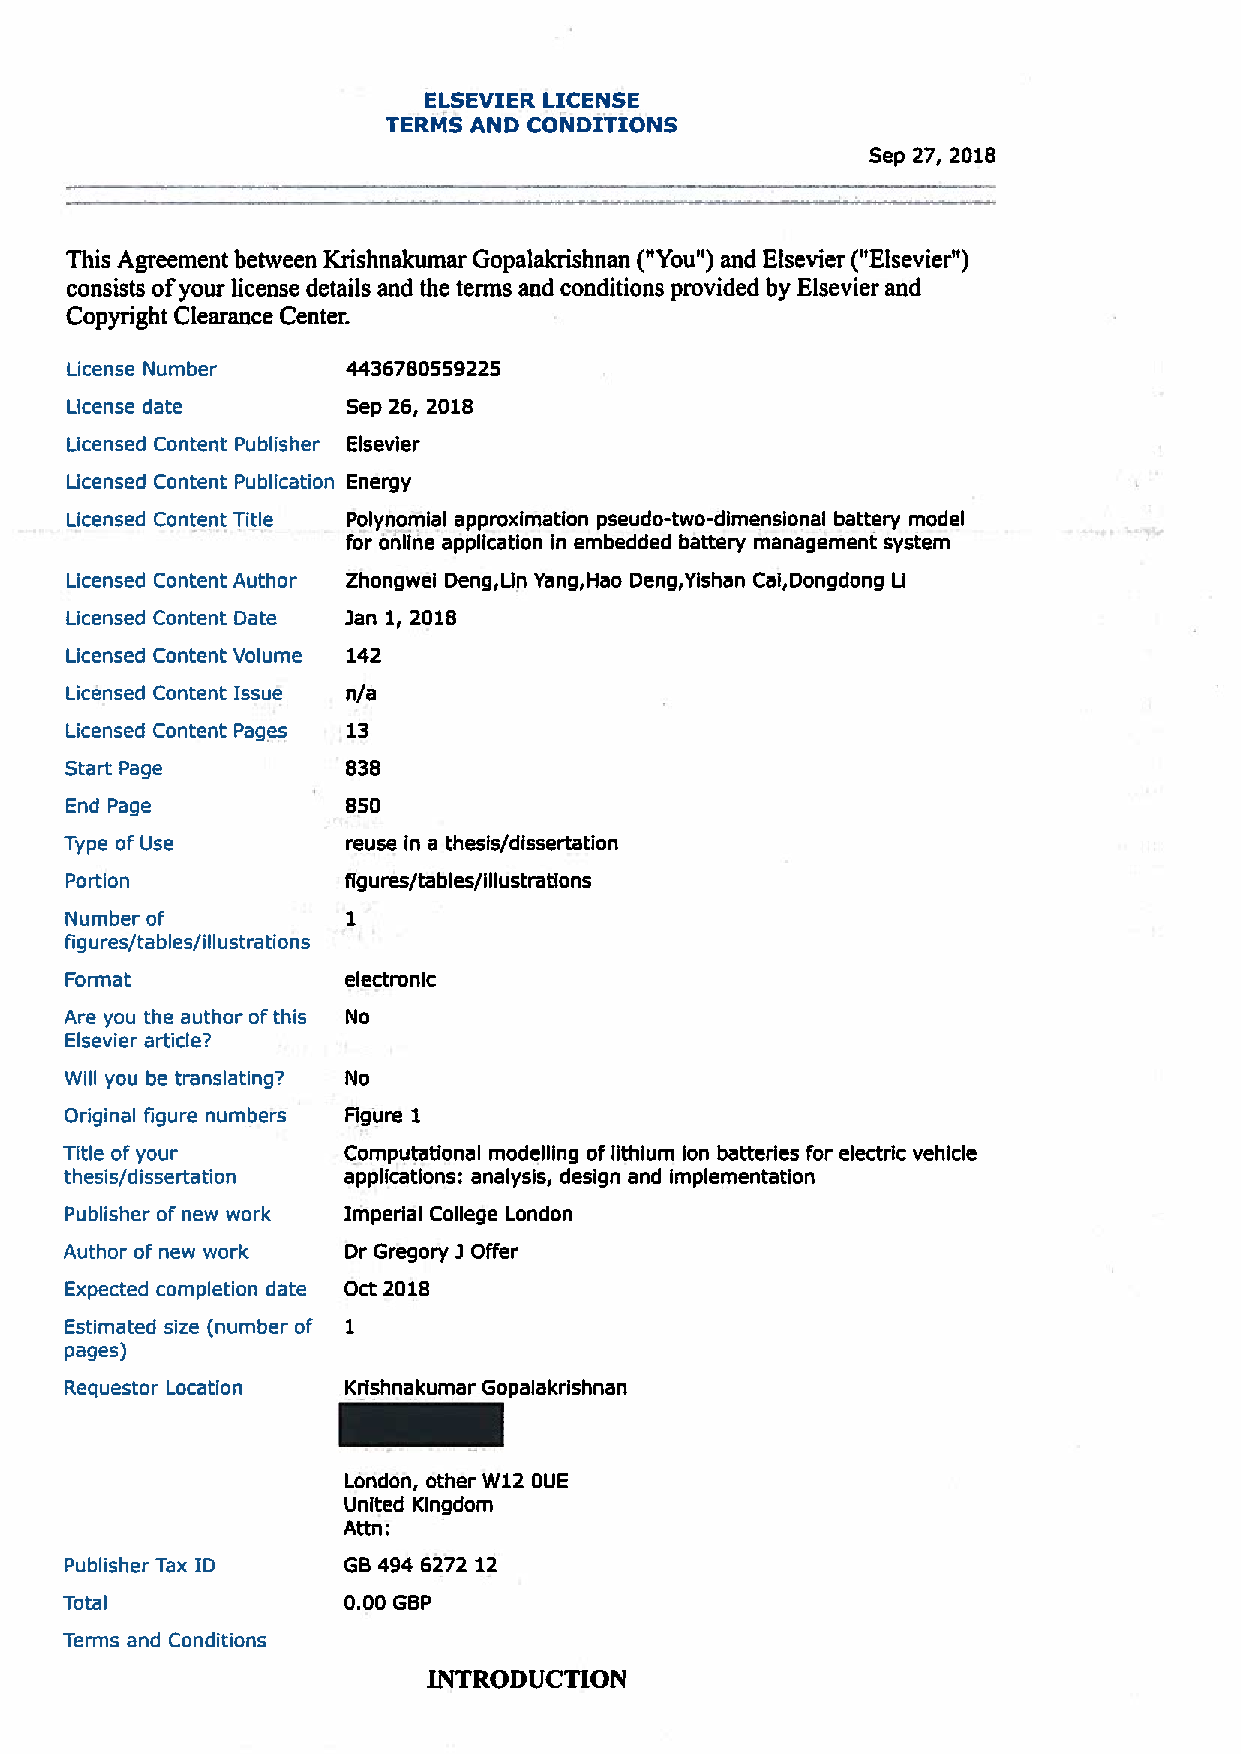
\includepdf[pages=-,scale=0.83,link,linkname=deng,pagecommand={\label{dengpermission}}]{backmatter/appendices/redacted_Deng_copyright.pdf}

\makeatletter\@sc@wm@stamptrue\makeatother


    % -*- root: ../../main.tex -*-
%!TEX root = ../../main.tex
% vim: nospell tw=80 fo=cqt

\setstretch{1.348361657291667} % golden-ratio stretch (1.2 x 1.348 = 1.618)
\chapter{Colophon}

This thesis was created using \LaTeXe and Bib\LaTeX{}. The corresponding source
code was edited in neovim using the vimtex plug-in. The typesetting engine used
is \StrBehind{\luatexbanner}{\detokenize{This is}}{}. The body copy is set in a
12pt Libertinus Serif text with the section headers set in Libertinus Sans. A
factor of 1.618 (golden ratio) is used as the spacing factor between any two
base-lines in the body copy. Source code listings are set in 9pt Latin Modern
Mono.

\end{appendices}


